
%%%% MACRO DEFINITION %%%%

\providecommand{\pvivax}{P.~vivax}
\providecommand{\pfalciparum}{P.~falciparum}
\providecommand{\cterm}{C-terminus}
\providecommand{\nterm}{N-terminus}

\providecommand{\e}[1]{\ensuremath{\times 10^{#1}}}
\newcolumntype{P}[1]{>{\centering\arraybackslash}p{#1}}
\newcolumntype{M}[1]{>{\centering\arraybackslash}m{#1}}

\providecommand{\refimage}[1]{\figurename~\ref{fig:#1}}

% figure that is as wide as the text
\newcommand{\insertfigure}[5][1]{
\begin{figure}[h!]
	\makebox[\textwidth]{\includegraphics[width=#1\textwidth]{Chapter1_pics/#2}}
	\caption[#3]{\small{#4}}\label{fig:#5}
\end{figure}
}

%TC:macro \note [ignore]



%%%%%%%%%%%%%%%%%%%%%%%%%%%%%%%%%%%%%%%%%%%%%%%%%%%%%%%%%%%%%%%%%%%%%%%%%%%%%%%%%%%%%%%%%%%%%%%%%%%%%%%%%%%%%%%%%%%%%
%%%%%%%%%%%%%%%%%%%%%%%%%%%%%%%%%%%%%%%%%%%%%%%%%%%%%%%%%%%%%%%%%%%%%%%%%%%%%%%%%%%%%%%%%%%%%%%%%%%%%%%%%%%%%%%%%%%%%
%													BEGIN
%%%%%%%%%%%%%%%%%%%%%%%%%%%%%%%%%%%%%%%%%%%%%%%%%%%%%%%%%%%%%%%%%%%%%%%%%%%%%%%%%%%%%%%%%%%%%%%%%%%%%%%%%%%%%%%%%%%%%
%%%%%%%%%%%%%%%%%%%%%%%%%%%%%%%%%%%%%%%%%%%%%%%%%%%%%%%%%%%%%%%%%%%%%%%%%%%%%%%%%%%%%%%%%%%%%%%%%%%%%%%%%%%%%%%%%%%%%

\chapter{Introduction} % Write in your own chapter title
\label{Chapter1}
\lhead{Chapter 1. \emph{Introduction}} % Write in your own chapter title to set the page header

Proteins are polymer chains of amino acid residues, and while the chemical diversity of the twenty canonical amino acids utilised in Biology can offer proteins a staggering variety of folds and functionality, there remain chemical processes that are not possible using only this chemical species. Consequently, many proteins use cofactors --- chemicals which associate with the protein but are not generally covalently bound to them.

In order for a protein to induce this association to happen, it must present a region of its surface to which the cofactor in question will experience an attraction, and for which association will be thermodynamically favourable. The residues that make up this attractive region are called binding sites.

Metal atoms are a common cofactor. In this case the binding site is a metal binding site, and when the metal is zinc, it is a `zinc binding site'.

Clearly, zinc will only experience an attraction towards certain kinds of protein surfaces, and so proteins which need to attract a zinc cofactor will have to present surface residues capable of doing this. It should be possible to predict, therefore, whether a protein's structure has a potential zinc binding site on it because only certain residues in certain geometric configurations will be capable of creating this high affinity for zinc. Furthermore, because structure is determined by amino acid sequence, it should in principle be possible to predict zinc binding capabilities from protein sequence.

This PhD project is an attempt to develop novel methods for doing so. Being able to predict whether a protein binds zinc from its sequence alone offers valuable insights into the function of the resultant protein, and allows entire genomes to be quickly searched for potential zinc binding proteins. Being able to predict zinc binding in a protein structure can reveal mechanistic information about how it carries out its function, as well as offering insights into how pathological zinc binding associated with that protein might be addressed. While there are previous methods for doing both of these things, this PhD project uses an entirely novel approach for doing so, backed by a comprehensive survey of all known zinc binding sites.

\section{Zinc}

\subsection{Cofactors}

Proteins are an expression of the information content of genetic material, and are the means by which the information content of that genetic material is effected. The translation process maps three-nucleotide codons to amino acids, building up proteins as polypeptide chains of some combination of twenty of these building blocks. These amino acids all contain the same atomic backbone, but each has its own unique side chain, and between them the twenty amino acid side chains cover a diverse range of chemical properties. There are hydrophobic and hydrophilic side chains, side chains of varied length, and varied electronic charge.

However, while this `polypeptide-space' is certainly vast, the different possible combinations and orientations of the twenty amino acid side chains still represent a small subset of total chemical space, and there are limits to what proteins can achieve using only these chemical species. The principal atoms involved (carbon, nitrogen, oxygen and sulphur) are all clustered at the upper right corner of the periodic table, all have broadly similar electronic properties, and are all similar in size.

Other regions of the periodic table are not available to evolution by the direct means of encoding them with DNA --- there is no codon that will cause them to be incorporated directly --- but these other chemical species can be incorporated through other means. The three-dimensional structure of a protein is determined by primary structure, so the genetic code can create a protein which presents a region of its surface that the `desired' (in the evolutionary sense) chemical species will be attracted to and will associate with the protein through non-covalent means (assuming it is present in the protein's environment). These are `cofactors'.

While there are many organic, molecular cofactors in use, metal ions --- particularly transition metal ions --- have particular properties that make them very useful as cofactors. To understand why this is, it will be necessary to briefly review the electronic structure of atoms, show how transition metals are distinguished by their particular electronic structure, and then look at how zinc's properties are unusual by the standards of other transition metals.

Atoms' electrons are arranged into energy levels, which are in turn sub-divided into orbitals - regions of space in which electrons will usually be found. For example, atoms can hold two electrons in the first, lowest energy level, which has a single s-orbital. The second energy level can hold eight electrons, with one slightly lower energy s-orbital and three slightly higher energy p-orbitals. This describes the electron arrangement of the first ten elements.

The third energy level is slightly more complicated. It has three sub-levels (an s-orbital, three p-orbitals, and five d-orbitals) but the d-orbitals are actually in a higher energy state than the s-orbital of the \emph{fourth} energy level, which `fills up' first. The order in which the orbitals fill up is therefore 1s2s2p3s3p4s3d4p and so on (see Figure~\ref{fig:orbitals}). An atom with thirteen electrons (i.e.\ aluminium) will have its thirteenth electron in a 3p orbital, an atom with nineteen electrons (potassium) will have its nineteenth electron in a 4s orbital, and only once an atom has to `add' a twenty-first electron (scandium) will the 3d orbitals be used.

\begin{figure}
\centering
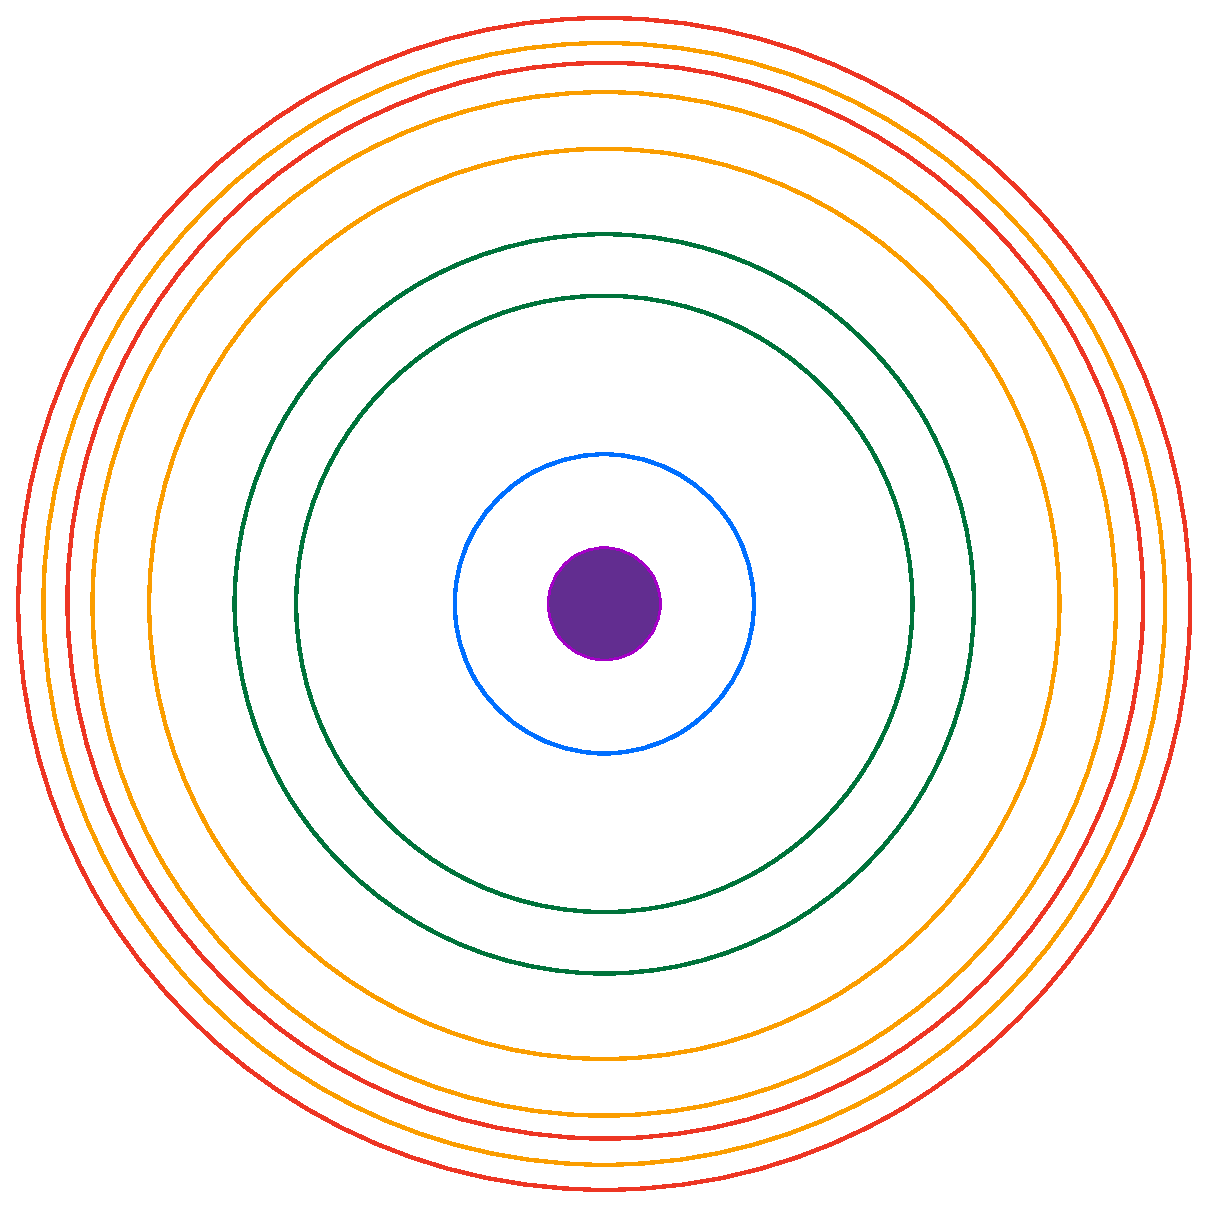
\includegraphics[width=1.0\textwidth]{Figures/orbitals.eps}
\caption[Stylistic representation of atomic orbitals]{\label{fig:orbitals} Stylistic representation of atomic orbitals, showing levels 1 (blue), 2 (green), 3 (orange) and 4 (red). The difference in energy levels becomes less pronounced further out, to the point where difference in orbitals within these levels becomes greater than those between them by level 4. It is for this reason that the highest energy orbitals of level 3 (3d) are higher in energy than the lowest energy orbitals of level 4 (4s). The distances shown here are not to scale with the actual energy differences.}
\end{figure}

Atoms which use these d orbitals --- the transition metals --- have unusual properties not encountered in previous atoms as a consequence. And it is precisely these properties that make them so useful to proteins, and why evolution has driven proteins to acquire them.

\subsection{Transition Metals}

Transition metals are often employed as cofactors by proteins, particularly in catalysis. As they occupy a different region of electron configuration space than the organic non-metal atoms that make up the biological amino acids (for reasons just outlined), they can provide functionality that would otherwise be unavailable.

Atoms `prefer' to have full energy levels and sub-energy levels --- in the sense that if they are in an environment which draws electrons away from them (an oxidising environment) it will be energetically favourable to lose whatever number of electrons causes them to fall back to the last filled level, emptying the highest energy level. Likewise, if in an electron-rich environment in which electrons are `pushed' to the atom (a reducing environment), they will prefer to take only the precise number of electrons which fills the current energy level.

For elements before scandium, this is straightforward: energy levels are far apart, and there is generally only one clear point to fall back to, or advance to. Sodium for example, has a single 3s electron, so when in an oxidising environment it can relinquish this one electron, and become Na+. It has a single oxidation state.

Once d-orbitals start being filled however, this becomes less straightforward. Rather unintuitively, when it comes to \emph{losing} electrons, different rules govern which energy levels are the first to be unfilled --- the 4s electrons can be considered the highest energy, and these will be lost first. Therefore most atoms with unfilled d-orbitals can adopt the 2+ oxidation state. The d-orbitals are rather close in energy level, so if there is further oxidative pressure, these can be lost too. This property of having multiple stable oxidation states is one of the chief characteristics of transition metals. It is partly for this reason that transition metals are so widely employed by evolution as protein cofactors, particularly in proteins which catalyse reactions --- enzymes. A common mechanism for catalysing a reaction is to stabilise an otherwise very thermodynamically unfavourable intermediate that might have a strong charge associated --- by using a chemical species which can have one oxidation state in its native state, but which will happily switch to a more oxidised form, the excess charge from the reaction intermediate can be temporarily `stored' in the cofactor, stabilising the intermediate.

As cations, the transition metals also act as efficient Lewis acids --- they can accept lone pairs of electrons. This is also useful in catalysis as it can stabilise intermediate structures by withdrawing excessive negative charge from them. This achieves a similar effect, but does so using a different mechanism. The metal atom is not being oxidised, however.

Another curious property of atoms with partially filled d-orbitals is the so-called breaking of degeneracy. In a single, uncharged atom of such elements, the five d-orbitals are said to be degenerate, in the sense of having identical energy levels. This is also true when oxidised, but when these charged ions interact with a solvent molecule or other ligands, some d-orbitals end up closer than others to the orbitals of the incoming ligand, entering a higher energy state than the others. The previously uniform d-orbitals split into two slightly different energy levels, and the previous degeneracy is said to have broken.

This confers some unique properties on these elements, most visibly that of colour. The electrons will prefer to occupy the lower energy d-orbitals, but the energy gap between them is small enough as to be in the visible light range, so light passing through a solution of these ions will have the corresponding wavelength absorbed, with the energy used to `promote' the electrons and with the light not absorbed determining the solution's colour.

It also means that different ligand geometries are associated with different changes in energy, meaning that certain geometries end up being preferred over others. This has implications for proteins, which must fold in such a way that the liganding residues adopt the correct geometry.

Unsurprisingly then, many proteins have evolved to take advantage of these useful properties of transition metals by presenting binding sites on their surface that will acquire one of them. This is generally done by bringing residues with available lone pairs into close proximity to each other, in an arrangement that matches the dimensions and orbital geometry of the desired metal, meaning that the geometric properties of these binding sites tend to match the particular properties of the metal atom they are adapted to. Each metal has its own particular properties arising from its electron configuration, and zinc's are some of the most atypical.

\subsection{Zinc's Unique Properties}

Though a transition metal in the sense that it has ten d-electrons but no 4p electrons, it is an unusual one, to the point where it is often not even classified as one\footnote{It is not particularly worthwhile to debate whether zinc is or is not a transition metal objectively --- transition metals are an artificial category invented to serve a particular purpose, and the edges of that category are blurred. By some definitions it is, but by other definitions it is not. What really matters are its objective physical/chemical properties, not the name of the category humans have assigned it to based on those properties.}. Many of the properties of transition metals derive from \emph{partially filled} d-orbitals, which zinc does not have. The five fully filled d-orbitals are relatively stable, meaning it can only really be oxidised to 2+ by losing its 4s electrons, so it has just one oxidation state. Electrons cannot be `promoted' from one d-orbital to another in solution as all spaces in the orbitals are already filled, so it has no colour or spectroscopic activity when in solution. At first glance, zinc would appear to be rather unremarkable metal, unworthy of much consideration by evolution.

However, the data shows otherwise. About 10\% of all proteins in the human genome are zinc proteins with a zinc binding site \cite{andreini2006counting} --- making it the second most abundant such metal after iron. It is also the only metal found in all classes of enzyme (hydrolases, oxidoreductases, lyases, transferases, ligases and isomerases) \cite{vallee1990zinc}. Clearly, evolution has found zinc very useful.

In fact it is precisely that unremarkableness that has made zinc so attractive. Having just one oxidation state may mean that it cannot hold onto an electron mid-reaction, but it also means that the ion will retain its electronic properties in a wide range of reducing environments, and its status as a particularly good Lewis acid means it is still very useful in catalysis. 

Its lack of spectroscopic activity may make zinc solutions colourless, but the same arrangement of d-orbitals that causes this also means that there is no energetic penalty for zinc coming out of solution (where it is octahedrally coordinated) and into the binding site because such a transition is accompanied by a rearrangement of the orbitals geometrically. In the case of metals with incomplete d-orbitals, more of the orbitals are forced into higher energy states. For zinc, there is no energetic penalty in moving from the octahedral geoemtry associated with solvation by water, to the (typically) tetrahedral geometry of protein binding. This equivalence in `Ligand Field Stabilisation Energy' gives zinc an advantage from the protein's perspective \cite{lachenmann2004zinc}.

As a somewhat unusual metal cofactor, the corresponding zinc binding sites that proteins form around them also have unique properties, distinct from those of other cofactors, and other transition metals. These will be explored next.

\section{Properties of Zinc Binding Sites}

What do zinc binding sites `look like' from a structural point of view? What are their properties at the atomic scale?

These questions were addressed by researchers from some of the very first crystal structures, and continue to be a topic of research today. The properties of zinc binding sites that distinguish them from other spatially proximate clusterings of residues are ultimately what must be used to predict them, so the advances in this field are crucial to any zinc binding prediction model. The history of our understanding of these properties will be reviewed here.

By the middle of the 1980s, a number of structures had been produced and already a few general themes that would recur over and over again were observed. Catalytic sites (those which are involved in the catalysis of some reaction) tended to have three protein ligands and one water ligand, whereas structural sites (those not involved in catalysis, but which stabilise local regions of the protein) generally had four protein residues, for example. One of the first reviews in this area to examine the structures obtained so far identified coordination by sulphur and nitrogen, and tetrahedral geometry, as the two defining characteristics of zinc binding sites \cite{williams1987biochemistry}. With the benefit of hindsight we can see that this is a slight simplification, but it shows that a consensus about `typical features' was beginning to form. Another early review would go on to list most of the basic properties of zinc binding sites we now know --- their division into structural and catalytic sites, the near ubiquity of water in catalytic sites, the much stronger preference for tetrahedral geometry in structural sites than in catalytic sites, and the preference for histidine, cysteine, aspartate and glutamate residues \cite{vallee1990zinc}. These properties would be repeated and elaborated upon by a number of similar reviews in this period \cite{tainer1991metal,vallee1992functional,coleman1992zinc}.

The more structures that were available, the more detailed the inferences that could be made became. A series of reviews looked at typical atom geometries in cysteine binding \cite{chakrabarti1989geometry} and histidine binding \cite{chakrabarti1990geometry}, and while both papers looked at metal binding generally rather than zinc, in both cases the observations were found to be largely metal-agnostic. It was shown that cysteine generally coordinated the metal such that the Zn---S-C$\beta$-C$\alpha$ torsional angle is either 90$^\circ$ or 180$^\circ$, and that histidine residues generally coordinate the metal via their NE2 nitrogen atom, with the metal lying in the histidyl plane.

Another structural characteristic of zinc binding sites (and indeed metal binding sites generally) was the `hydrophobic contrast' that seemed to exist around them \cite{yamashita1990metal,gregory1993prediction}. Briefly, this is the observation that metal atoms in a protein tend to be surrounded by a shell of hydrophilic atoms (as might be expected), but that these were in turn surrounded by unusually hydrophobic atoms (measured against the average `background' hydrophobicity of the other residues). This could be implemented as a function of coordinates, which would be at a maximum when centered in such a concentric sphere. It was shown that maxima of this function would cluster around metal binding sites.

Whilst it might be expected that zinc binding sites would have some kinds of structural consensus, it is not immediately obvious that they should have any kind of predictable sequence patterns. However in 1989 it was shown, albeit from a relatively small dataset as existed at that time, that catalytic zinc binding sites seemed to have characteristic ``short and long spacer sequences" \cite{vallee1989short}. That is, the three residues that make up catalytic binding sites seem to be made up of two residues separated by a small stretch of amino acids (around five) and a third residue that is much more distal on the sequence. They proposed that the first two residues were acting as a nucleus, a proto-site that is stabilised by the third residue. This pattern was confirmed by later studies, with the short spacer being found to be generally 2 to 7 residues long \cite{patel2007analysis}.

This was not however the \textit{first} sequence motif associated with zinc binding sites - a few years previously a curious pattern of residues in a transcription factor sequence led to the discovery of a new class of zinc protein, and the creation of a entirely new field of genome engineering.

In 1985 it was observed that a particular transcription factor in the model organism \emph{Xenopus laevis} was a zinc protein, and moreover that it seemed to be made of globular subunits of roughly equal mass, each with a repeating C...C...H...H motif \cite{miller1985repetitive}. They hypothesised that perhaps this particular transcription factor was essentially a string of zinc binding domains --- referred to as `fingers' --- each stabilised by a zinc atom at the base. The very regular repeating pattern of thirty residues, each with these four residues in the same location, was key in uncovering these `zinc fingers'. While not initially thought to be widespread, in the months and years that followed, more examples of these genome-interacting proteins with similar sequence motifs were identified \cite{payre1988finger}. Finally, in 1989, the structure of the original zinc finger was solved, largely confirming the initial speculations about the structure of this protein, and the role of zinc within it --- the domain was a finger-like projection which could bind DNA bases at the tip, and which was stabilised by a C2H2 zinc binding site at the base.

The field continued to grow. By 1998 there were thought to be at least 500 zinc finger proteins, and possibly as many as 1\% of all mammalian genes \cite{mackay1998zinc}. Much of this field is concerned with the `fingertip' end of zinc fingers, which actually implements the DNA-recognising properties, though for the purposes of this project it is the base that is of more interest. There are a few points to take away from this brief digression. The first point, which will be returned to in the section on zinc binding site prediction, is that the zinc fingers were discovered because of a characteristic \textit{sequence} pattern, emphasising that such prediction is both possible and potentially offers many insights. The second is that until this point, much of the interest in zinc binding sites was in catalytic zinc binding sites; there were fewer structural sites available to study, and most reviews from this period addressed them last, if at all. From this point on however, many more became available to study, and it became clear that they were responsible for much of zinc's ubiquity across the proteome.

Most of the early work on characterising the typical properties of zinc binding sites was done by manually surveying the crystal structures available and drawing conclusions from them. But as the 1990s wore on and the number of such structures available reached the hundreds, this became increasingly impractical. Instead, from this point onwards, the sites would have to be collated algorithmically from the Protein Data Bank \cite{berman2000pdb}.

The first such database survey was in 1998. They found 387 zinc proteins, and after excluding some on quality and experimental technique factors, they were left with 111 \cite{alberts1998analysis}. Some of their findings were in line with what was already known: the three residue/one water combination for catalytic sites, the preference for tetrahedral geometry, histidine's preference for one nitrogen over another (by a ratio of 70:30, they found). They also identified a new, almost ubiquitous, motif across zinc binding sites which they call the `elec-His-zinc' motif whereby zinc is liganded by a histidine which in turn forms a hydrogen bond with an electron donor of some kind.

This was followed by other reviews \cite{roe1999zinc,laity2001zinc,grishin2001treble,harding2001geometry,krishna2003structural}, showing similar results: that zinc-ligand distances are similar to those found in small molecules, and further sub-categorising the ever increasing number of zinc finger proteins.

Increasingly, the modes of classification were becoming more sophisticated too. Initially, two kinds of binding site were recognised: catalytic sites, which catalysed some metabolic reaction, and structural sites, which did not and just stabilised structure. Later came the recognition that some sites required the action of multiple metals in a single functional unit --- either multiple zinc atoms, or a zinc atom in conjunction with another metal atom. From 2001, a fourth kind was recognised, interface binding sites \cite{auld2001zinc}. It had been known since the early days of insulin research, of course, that in some cases zinc atoms could stabilise polymeric structures, but by this point there was enough data to classify these as their own category, with their own properties --- that cysteine is very underrepresented in them, that stabilisation is often done by beta sheets rather than alpha helices (common in other zinc binding sites), and even evidence that these sites could also have catalytic roles in addition to their role in quaternary structure.

A more in-depth look at the differences between catalytic and structural sites even seemed to offer a means of automatically classifying zinc binding sites \cite{lee2008physical}, though generally during this period this was a task done manually. They confirmed that catalytic zinc binding sites tended to have more unusual atom distances and geometries (imposing a `strain' upon them that we will return to in the following section), and looked in detail at catalytic sites' disdain for cysteine residues. They found that a relatively simple method of assuming a site is structural if it has more than one cysteine residue \textit{and} no water, and assuming it is catalytic otherwise, assigned the correct label in 90\% of cases in their dataset. They also looked at the possibility of using atom distances to classify zinc binding sites, though it must be remembered that when looking at differences in atom distance on the order of single {\AA}ngstr\"{o}ms, structure with poor resolution should be removed from the dataset if you are to make sensible inferences.

Atom distances themselves have been a major focus of research. A typical example is a 2007 review of 994 structures \cite{tamames2007analysis}, showing that histidine approaches zinc more closely than cysteine (2.11 \AA \ versus 2.32 \AA \ on average) with water distances generally somewhere between those two figures. The vast majority of metal liganding atoms are within 3 {\AA} of the metal \cite{dokmanic2008metals}. It has been speculated that some non-zinc metal-ligand distances are longer than might otherwise be expected because of the `Jahn-Teller effect' \cite{doi:10.1002/prot.21601}. This phenonemon, like the Ligand Field Stabilisation Energy that makes zinc so attractive in the first place, results from the different energy levels of the d-orbitals in these metals which distorts them and lengthens the bond. This does not affect zinc binding, but does affect other metals.

The properties of zinc binding sites are not just limited to the metal itself and the residues that coordinate it. It is increasingly recognised that the `secondary shell' around the primary residues are of great importance, by providing a network of stabilising hydrogen bonds around the liganding residues to keep them in their precise orientation \cite{auld2001zinc}. This concept has been extended to the idea of a `Minimal Functional Site' \cite{andreini2011minimal}, proposed as the smallest unit of metal binding that should be used when classifying and studying the phenomenon. The authors in this case used all residues within 5 \AA \ of a liganding residue, but more important is the general idea that the residues around the coordinating residues, which are often part of secondary structure, are crucial to understanding the metal binding itself.

There have also been reviews into the efficacy of these database reviews at all, and the limits of what can be inferred from them. A 2005 review \cite{sommerhalter2005x} suggests that while purely spatial properties, such as the location of the metal ion and its liganding residue identities, can be provided reliably by crystallography, often the precise coordination geometry does not agree with spectroscopic data, and should be treated with caution. They also warn against trying to infer redox state from crystallography, though this does not particularly apply to zinc. A later review \cite{laitaoja2013zinc} pointed out that reported atom distances increase as a function of resolution, and stresses the need to take this into account. They criticise a number of earlier studies for treating unlikely geometries or electronic configuration as `real', or for treating zinc salts and crystallographic artefacts as biologically relevant zinc binding sites.

Finally, it is worth examining the numerous secondary databases that have been created over the past decade and a half relating to zinc binding sites, and which offer a web-accessible means of viewing the properties of zinc (though usually metals generally) binding sites.

\begin{itemize}

\item MESPEUS was one of the first --- a general-purpose database of metal binding sites generally, which focused on providing basic geometric information \cite{hsin2008mespeus}, and which allowed basic surveys of atom-length patterns to be carried out.

\item ZifBASE had a more specific focus --- this was a database of zinc fingers specifically, and provided much more than structural information from the PDB: sequence information, DNA targets, and physiochemical properties like isoelectric point were also provided \cite{jayakanthan2009zifbase}.

\item Probably the most important resource in this area is MetalPDB \cite{andreini2012metalpdb}, a database of metal binding sites, similar to MESPEUS, but with more information and a more sophisticated means of classifying them. They divide their sites into `equistructural sites' - (those which have binding sites of similar structure) and within those `equivalent sites'  (equistructural sites with the same metal). They place a great focus on the secondary shell, as part of the `Minimal Functional Site' concept they introduced earlier, and have recently updated the resource with a greater focus on apo-structures \cite{putignano2017metalpdb}. They have also provided a number of related resources, such as MetalS3 \cite{valasatava2014metals}, a tool for searching the database via structure pattern rather than keyword, and tools for classifying sites based on similarity \cite{sobolev2013web}. An issue with MetalPDB however is its reliance on asymmetric units in the PDB files they parse. Often the raw coordinates of such files represent only the repeating unit of the crystal structure, and the actual `real' biological protein must be assembled from that data using transformation matrices contained with the files. MetalPDB (and most other resources) do not do this, which makes some of their `binding sites' rather unrealistic.

\end{itemize}

Another impression one gets immediately when surveying these resources is that with the exception of MetalPDB, all of these resources have ceased to exist --- their URLs go nowhere, or their sites are broken beyond reasonable use and obviously not maintained. This is a problem generally with academic software, in which the creation of resources is funded by initial grants. However, because they do not generate revenue themselves, they need grant funding of some kind in perpetuity if they are to remain online --- which they generally do not have. The solution to this problem is not obvious, and in any case beyond the scope of this PhD, though the burden that this maintenance poses for a lab or organisation can be lightened somewhat by automating as much of the process as possible (where appropriate).

Other resources are focused more on validating or describing a given metal binding site that it is presented with, such as the coordination geometry classifier FindGeo \cite{andreini2012findgeo}, or the validation tool CheckMyMetal \cite{zheng2017checkmymetal}, which uses known properties of metal binding sites to determine if a proposed binding site is realistic.

\section{How do Zinc Binding Sites Work?}

In parallel with an increasingly clear understanding of the properties of zinc binding sites, theoretical and analytical research has been performed on the mechanisms and physics underpinning zinc binding. These two areas of research are complimentary and interconnected, with the properties in large part explained by the physics of the binding sites, and insights into the mechanisms derived from experimental observations.

One of the earliest concepts to be introduced in this area was that of the `entatic state' of metals in biology \cite{vallee1968metalloenzymes}, in the 1960s. Essentially this was the idea that metal atoms in proteins have different geometries and properties than they do in smaller molecules and which they would `prefer' energetically, because the protein backbone is able to impose restraints upon it. It is a kind of `strain' that the protein's overall conformation imposes on the metal and which gives the metals any unique properties they may posses which are not found outside of biology. For example, it may cause an otherwise unfavourable metal oxidation state to be favoured over another, as can be seen with iron.

This concept was later elaborated upon to show that this strain should be thought of as a two-way process \cite{williams1985symbiosis}. The authors note that ``[They] described the valuable strains induced by the protein in the metal... but they could equally well have pointed to the strain induced in the protein by the metal to it. The overall idea was that of catalytic perfection induced by strain" --- a strain which makes the enzyme ``energetically poised for catalysis" \cite{vallee1984metallobiochemistry}.

This is a concept that applies to metalloproteins, but once it started to become apparent just how widely used zinc was in the 1980s, attention began to turn to answering the question of why zinc in particular was of such apparent use to proteins.

One property noted early on was that zinc atoms have a full \textit{d}-shell, making it slightly unusual among transition metals\cite{vallee1984metallobiochemistry}. This means that when ionised, zinc will lose its two 4\textit{s} electrons to become 2+, but there are no other oxidation states that it can realistically adopt --- it is `redox inert'. This means that the protein can rely upon the metal retaining its oxidation state regardless of the oxidation environment it finds itself in, a stability whose utility is clear.

Another property of this full d-shell that would be elaborated upon later was the absence of a phenomenon known as `ligand field stabilisation energy' \cite{lachenmann2004zinc,vahrenkamp2007does,maret2009coordination,krkezel2016biological}, as previously outlined. Briefly, this refers to the fact that atoms with incomplete d-shells, like most other transition metals, have preferred coordination geometries and experience energetic penalties if coordination angles deviate from this. If the d-shell is full however, no one geometry is preferred over another, which offers the protein much more flexibility.

Another property of zinc that is revisited time and time again in the literature is zinc's role as a Lewis Acid; it will readily accept electron pairs from electron pair donors \cite{williams1984zinc}. It has been noted that while other metals are superior Lewis acids from a purely chemical standpoint, zinc will more readily form tetrahedral complexes \cite{bertini1985zinc}, making it frequently the Lewis acid of choice.

This effective electron-pair-accepting that zinc exhibits is important because it is useful wherever zinc is used in catalysis. One of the first zinc enzymes to have its precise mechanism of action investigated was carboxypeptidase A, a digestive enzyme. It was suggested that the water molecule that coordinated zinc as one of its ligands was being `activated' by zinc --- its electron pairs were being withdrawn by the metal, making it less able to retain its hydrogens and becoming the more reactive hydroxide. Some structural evidence to support this came from the crystal structure of carboxypeptidase A in complex with a substrate that was known to be hard for the enzyme to digest for reasons at that time unknown. The crystal structure revealed that the substrate was inadvertently looping around and coordinating the zinc atom, blocking the water molecule and accounting for the much slower rate of hydrolysis \cite{christianson1986x}. Another means by which zinc can aid in catalysis is by stabilising any negatively charged intermediate in the reaction by offering a temporary repository for their electrons, as is the case with carbonic anhydrase \cite{christianson1996carbonic}.

Indeed, multiple papers have emphasised this `primed' property of catalytic zinc sites. They have more distorted geometry than the more typically tetrahedral structural sites \cite{roe1999zinc}, the liganding atoms tend to be further from the metal \cite{lee2008physical}, and they are generally more thermodynamically unfavourable when modelled quantum mechanically \cite{sousa2009zinc}.

The means by which protein residues interact with the metal can also have important consequences. Aspartic acid and glutamic acid are both relatively common zinc binding residues, each doing so via their side chain carboxylate groups. They can either contribute one liganding oxygen atom (`monodentate' binding) or both (bidentate binding) (see
Figure~\ref{fig:carboxylate}). While early theoretical models suggested that the different modes were determined merely by the other residue identities, with more negative other residues favouring mere monodentate binding \cite{ryde1999carboxylate}, it has more recently been suggesting that a residue may use both. The so-called `carboxylate shift' is theorised to occur when an acidic side chain in a catalytic zinc binding site switches from monodentate binding to bidentate binding so as to keep the number of coordinating atoms around the zinc constant, and thereby reducing the activation energy of substrates entering and leaving the complex \cite{sousa2007carboxylate}.

\begin{figure}
\centering
\includegraphics[width=1.0\textwidth]{Figures/carboxylate.eps}
\caption[Monodentate and bidentate binding]{\label{fig:carboxylate} A zinc binding site demonstrating both bidentate binding via two glutamate residues, and monodentate binding via one aspartate residue. This visualisation is taken from ZincBind (binding site 6VDA-1), and is a site in PDB 6VDA, a \emph{Thermotoga maritima} transport protein \cite{udagedara2020pdb}.}
\end{figure}


The reason for the preference for cysteine in structural sites has also received attention. It has been proposed that cysteine residues transfer more charge to the zinc atom, reducing the potency of its 2+ charge and making it less reactive \cite{lee2008physical}. 

Finally, it is worth bearing in mind that zinc does not become `part' of the protein as part of the translation process, but binds to the fully translated apo-protein, in a process whose mechanisms are also crucial to understand. It is possible to compare the apo- and holo-forms of zinc binding proteins using sequence identity. For every zinc binding protein structure you have, you can search the Protein Data Bank for proteins with a highly similar structure that does not have zinc in the same position. This is precisely what a 2005 review did \cite{babor2005flexibility} in a bid to investigate the mechanisms by which zinc binds proteins in the first place. After looking at 210 apo/holo pairs, they found that often, at least part of the coordination shell is in place before the metal is in place. This is consistent with the `nucleus' theory of the short and long spacer sequences, outlined above. Furthermore, they found that in just 40\% of cases was there any rearrangement of side chains upon metal binding, and in just 14\% of cases did this involve backbone rearrangement. This mode of zinc binding is encouraging for efforts to predict zinc binding from apo-structure, as we will see in the next chapter.

This zinc binding should also not be thought of as permanent. Metalloproteins are in equilibrium with free metal + apoprotein, and the zinc binding will have an on and off rate like any other complex. While this project is largely focused on proteins where the zinc is essentially a permanent feature of the protein because it is essential for some function, it has been pointed out that these are merely proteins where the equilibrium is far to the right, and that all metal proteins lie on a continuum in this regard, with zinc transporters (for example) having an equilibrium further to the left \cite{maret2010metalloproteomics}. This equilibrium constant is determined by the geometry of the binding site, and the secondary shell around the liganding residues seem to play a very large role in fine-tuning this affinity by exercising careful control over the precise positioning of these side chains \cite{kochanczyk2015relationship}.

\section{The Protein Data Bank}

The ultimate data source for almost all the data used in this project is the Protein Data Bank (PDB) \cite{burley2020pdb}. This is a Bioinformatics Database jointly administered by the Research Collaboratory for Structural Bioinformatics (RCSB), the Protein Data Bank in Europe (PDBe) and Protein Data Bank Japan (PDBj) --- each a member of the overarching Worldwide Protein Data Bank (wwPDB). These organisations accept depositions of solved protein structures from researchers around the world, releasing them as PDB structure files with four character IDs. There are over 160,000 structures available in the PDB in 2021.

These `solved structures' contain the three-dimensional coordinates of the atoms that make up a macromolecular structure --- typically a protein or protein complex, often with small molecules bound, but there are nucleic acid structures in the Data Bank too, and increasingly large ribosomal structures. The structure files also contain meta-data about the experiment which produced the raw data from which the coordinates were calculated, details of any refinement done to those coordinates, and annotations of the names and entity relationships of the molecules present (which residues belong to which polymer, which small compounds have binding sites in which polymer, which molecules are instances of the same biological entity, etc.).

These three-dimensional coordinates are obtained by isolating the protein in question, performing some kind of experimental, analytical technique on the sample, and inferring the locations of the atoms from that data.

\begin{itemize}

\item By far the most common technique used is X-ray Diffraction. The sample is crystallised such that the structure arranges itself in a single, solid repeating lattice, and then X-rays are passed through this structure. This beam of electromagnetic radiation is diffracted by the atoms of the structure and, because the proteins are all aligned, this diffraction will create a discrete `diffraction pattern' of spots on the photoreceptive surface behind the sample. Specifically it is electron density which scatters the X-rays, and it is this which is detected. This pattern of spots can be used to generate an inferred three dimensional map of electron density by using Fourier Transforms, from which the location of the atoms themselves can be `fit'.

\item Nuclear Magnetic Resonance (NMR) spectroscopy is another technique used to generate atomic coordinates. Here the sample is placed into a very strong magnetic field, which causes the quantum spin of the atoms' protons to align with this field. Pulses of radio waves are then passed through the sample, which temporarily aligns the spin of the atoms with this electromagnetic radiation. When they relax back into alignment with the magnetic field, they emit radio waves which are detected, and which can be used to infer the proximity of the different atom types in the sample. This contains enough information to build up a map of atom connectivity, and from this atomic coordinates.

\item An increasingly prevalent technique is Cryo-Electron Microscopy (Cryo-EM). Rather than holding proteins in place by crystallising them into a repeating lattice and inferring their coordinates using X-Rays, they are `flash frozen' by rapidly lowering the sample's temperature, and then probed with beams of electrons.

\end{itemize}

Despite the increasing rate of submission of Cryo-EM structures, the majority of structures considered in this project have still been solved with X-Ray Crystallography.

The field of structural biology is diverse, but there are a number of concepts from this field and the protein structures mentioned above which are of particular importance to this project.

\begin{itemize}

\item Resolution. Typically given in ~{\AA}ngstr\"{o}ms (0.1 nm), this is a single value metric of the quality of a protein structure. It is essentially a measure of how `detailed' the electron density map is. High resolution structures (confusingly these are those with lower values, around 1 ~{\AA}ngstoms) might detect the contours of individual atoms within a protein residue for example, whereas lower resolution structures (higher values, above, say, 3 ~{\AA}ngstr\"{o}ms) might merely have residue-shaped blobs. In analyses where the coordinates of atoms need to be relied upon with reasonable precision, a common early step on the pipeline is to discard structures with resolutions below some threshold.

\item R-values. Another single-value that represents the quality of a protein created from X-Ray Diffraction. Part of the process of generating an electron density map from a scattering pattern is an iterative process whereby the researcher creates a putative set of coordinates, calculates what pattern of scattering would theoretically correspond to those coordinates if they were accurate, compares this with the actual scattering map, and refines the coordinates based on the difference. This difference between the actual scattering pattern, and the scattering pattern that would produce a given set of coordinates, is the R-value. A perfect match would be 0, but typical values are around 0.2. A distinction is usually made between these R-values, and `free' R-values, in which around 10\% of the observations are removed before refinement, and then the refinement is performed on the remaining 90\%, with the free R-value a measure of how well the new simulated diffraction pattern predicts the remaining 10\%.

\item Temperature factors. The above metrics apply to an entire structure, but the quality of a set of coordinates might be better in some regions than others. Temperature factors represent this localised quality, as each atom has its own temperature factor. They are a measure of the uncertainty over the atom's position in space, with higher temperature factors indicating greater uncertainty (representing either statistical uncertainty regarding where the atom is likely to be, or actual variation in the atom's location due to excitation --- hence the name `temperature factors'). This uncertainty can be a single value `isotropic' temperature factor (applying in all directions) or `anisotropic' (directional uncertainty).

\item Biological Assemblies. The raw coordinates of PDB structures as given contain the `Asymmetric unit', which is the repeating unit of the solved structure. This may not be the actual biologically relevant entity, so a number of assemblies are generated computationally using this base unit, and their biological feasibilities calculated from metrics such as buried surface area and the interaction strength of associated surfaces. These possible assemblies are given in the metadata of the PDB files as transformation matrices, along with the associated software-calculated metrics.
\end{itemize}

\section{Conclusion}

Zinc is a crucial metal for a wide variety of functions in biological systems, and across a wide spectrum of organisms. Its chemical properties --- particularly its lack of redox activity which gives it an essentially permanent 2+ charge in physilogical environments regardless of the reducing/oxidising environment it finds itself in --- make it uniquely useful to proteins in carrying out functions that they would be unable to do with either the chemistry of the twenty canonical amino acids (whose atoms are largely electron donors, not acceptors), or other transition metals (whose redox state can alter depending on the environment). Chiefly those functions are the catalysis of reactions as a key component of enzymes, or as a stabiliser of local protein structure --- either a region of a single chain, or at the interface between two chains.

While zinc has other occasional roles, such as as a cellular messenger, these two primary roles require the zinc ion to be tightly and permanently bound to the protein in question. This requires the protein to fold in such a way that it brings together liganding residues for zinc that the metal will have a strong affinity for, due to the geometry and chemical identity of the atoms in question. These zinc binding sites have been examined in every greater detail as the number of zinc protein structures has increased, and certain key properties of the binding sites have been observed repeatedly at both the sequence and structure level.

Some of these characteristic features are the overwhelming use of histidine and cysteine, and to a slightly lesser extent the carboxylate residues aspartate and glutamate (with cysteine being more common in structural sites and the carboxylate residues slightly more common in catalytic sites), the near ubiquity of tetrahedral geometry of the liganding atoms, the presence of three liganding residues plus water in catalytic sites and four residues in structural sites, and the typical liganding distances.

Physically, the zinc binding sites seem to rely heavily on a network of stabilising hydrogen bonds holding the primary liganding residues in place, from the secondary residues around them. Binding between the zinc atom and the binding site does not usually rearrange the backbone of the protein signficantly. Zinc largely facilitates catalysis by stabilising the negative charges of any positively charged reaction intermediates, making their existence less thermodynamically unfavourable for the short amount of time that they exist.

The existence of these typical features and well understood mechanisms of action is crucial in trying to predict zinc binding sites from structure or sequence, as it means that there are particular properties to be looked for. The next chapter will examine the methods for making these predictors, and review previous attempts at predicting zinc binding using these techniques.


%\insertfigure[0.5]{name.eps}{short caption}{long caption}{label}
% N.B. do not \end{document} at the end of the chapters
